%% 
%% Copyright 2019-2024 Elsevier Ltd
%% 
%% This file is part of the 'CAS Bundle'.
%% 
%% It may be distributed under the conditions of the LaTeX Project Public
%% License, either version 1.2 of this license or (at your option) any
%% later version.
%% 

\documentclass[a4paper,fleqn]{cas-dc}

\usepackage[numbers]{natbib}
\usepackage{booktabs}
\usepackage{amsmath,amssymb}
\usepackage{graphicx}
\usepackage{url}
\usepackage{hyperref}
\usepackage{multirow}

\begin{document}
\let\WriteBookmarks\relax
\def\floatpagepagefraction{1}
\def\textpagefraction{.001}

\shorttitle{PatchXFormer: Enhanced Transformer for Solar Power Forecasting}
\shortauthors{C. Karunathilaka and S. Wickramanayake}

\title[mode = title]{PatchXFormer: Enhanced Transformer Architecture for Long-Term Solar Power Generation Forecasting}

\author[1]{Chathushka Karunathilaka}
\ead{chathushka.23@cse.mrt.ac.lk}
\credit{Conceptualization, Methodology, Software, Validation, Formal analysis, Investigation, Data curation, Writing -- Original draft, Visualization}

\author[1]{Sandareka Wickramanayake}
\cormark[1]
\ead{sandarekaw@cse.mrt.ac.lk}
\credit{Conceptualization, Methodology, Supervision, Writing -- Review and editing}

\affiliation[1]{organization={Department of Computer Science and Engineering, University of Moratuwa},
                city={Moratuwa},
                country={Sri Lanka}}

\cortext[cor1]{Corresponding author}

\begin{abstract}
Accurate long-term solar power generation (SPG) forecasting is essential for optimizing renewable energy integration into electrical grids and supporting effective energy management. However, the variability driven by meteorological factors and the non-linear relationships inherent in SPG data make accurate long-term forecasting challenging. This paper proposes PatchXFormer, a novel Transformer-based architecture specifically designed for SPG forecasting. PatchXFormer incorporates four key innovations: enhanced patch embedding with global tokens, frequency-enhanced attention combining temporal and frequency-domain analysis, adaptive normalization for robustness across diverse conditions, and cross-attention mechanisms for effective meteorological feature integration. We evaluate PatchXFormer using four real-world datasets from distinct geographic regions, including three new datasets from Sri Lanka (tropical climate) and one from the USA (temperate climate). Experimental results demonstrate that PatchXFormer achieves superior performance compared to seven state-of-the-art baselines, with improvements of 6.1\% to 5.4\% in Mean Squared Error across forecasting horizons of 24 hours to 7.5 days on the primary dataset. A comprehensive ablation study validates architectural choices, revealing that cross-attention for exogenous feature integration provides the largest performance gain. Cross-geographic evaluation uncovers significant geographic generalization challenges, while intra-country evaluation demonstrates robust generalization within similar climatic conditions.
\end{abstract}

\begin{graphicalabstract}
\includegraphics{graphical_abstract.pdf}
\end{graphicalabstract}

\begin{highlights}
\item PatchXFormer: novel Transformer with frequency-enhanced attention for solar forecasting
\item Three new tropical solar power datasets from Sri Lanka addressing data scarcity
\item Cross-attention for weather integration yields largest ablation improvement
\item Cross-geographic evaluation reveals asymmetric generalization patterns
\item Outperforms seven baselines across all forecasting horizons (24h to 7.5 days)
\end{highlights}

\begin{keywords}
Solar power forecasting \sep Transformer \sep Time series forecasting \sep Deep learning \sep Patch embedding \sep Frequency attention
\end{keywords}

\maketitle

\section{Introduction}\label{sec:introduction}

Solar power has emerged as a critical component of the global energy portfolio, offering a renewable and sustainable solution to growing energy demands. However, the inherent variability and intermittency of solar power generation (SPG) pose significant challenges for grid operators and energy management systems. Accurate forecasting of SPG is imperative for optimizing solar energy integration into electrical grids, reducing reliance on backup power sources, and improving the economic viability of solar installations~\cite{ahmed2020review}.

The challenge of solar power forecasting stems from the complex interplay of meteorological conditions---cloud cover, temperature, humidity, atmospheric pressure, and wind patterns---as well as temporal patterns related to diurnal cycles and seasonal variations. Over the past decades, methodologies have evolved from traditional physical models based on Numerical Weather Prediction (NWP) to statistical approaches and advanced deep learning algorithms~\cite{ahmed2020review,han2019review}. Deep learning approaches, particularly Transformer-based architectures~\cite{vaswani2017attention}, have shown remarkable success in time series forecasting, offering potential to capture complex non-linear patterns.

Recent Transformer-based models such as PatchTST~\cite{nie2022patchtst}, Informer~\cite{zhou2021informer}, and Autoformer~\cite{wu2021autoformer} have demonstrated state-of-the-art results in long-term time series forecasting. However, their application to SPG forecasting remains under-explored, particularly for diverse geographic locations and extended forecasting horizons. Furthermore, most existing SPG datasets contain synthetic data~\cite{ECMWF,GFS,SoDa,SARAH} that may not reflect real-world challenges, and datasets from tropical regions are notably limited.

Several critical limitations exist in current approaches: (1) long-term forecasting accuracy declines significantly as horizons extend beyond short-term predictions; (2) models trained on one geographic region demonstrate poor generalization to different regions; (3) the optimal utilization of meteorological features remains underexplored; and (4) models struggle to maintain consistent performance across varying environmental conditions.

This paper addresses these limitations by proposing PatchXFormer, a novel Transformer-based architecture specifically designed for SPG forecasting. The key contributions are:

\begin{enumerate}
    \item A novel architecture incorporating enhanced patch embedding with global tokens, frequency-enhanced attention mechanisms, adaptive normalization, and cross-attention for exogenous feature integration.
    
    \item Three new real-world SPG datasets from Sri Lanka (tropical climate), addressing the critical gap of limited tropical region data.
    
    \item Comprehensive evaluation across multiple datasets, geographic regions, and forecasting horizons, including cross-geographic and intra-country generalization analysis.
    
    \item A systematic ablation study validating architectural design choices, with detailed feature importance analysis.
\end{enumerate}

The remainder of this paper is organized as follows. Section~\ref{sec:related_work} reviews related work. Section~\ref{sec:methodology} presents the PatchXFormer architecture. Section~\ref{sec:experiments} describes the experimental study. Section~\ref{sec:discussion} discusses findings. Section~\ref{sec:conclusion} concludes the paper.

\section{Related Work}\label{sec:related_work}

\subsection{Solar Power Forecasting Methods}

Solar power forecasting methods can be categorized into traditional approaches, machine learning methods, and deep learning architectures. Traditional methods include physical models based on NWP~\cite{de2006improvement,rahman2015effects} and statistical models such as ARIMA~\cite{box2015time,singh2019guide,colak2015multi}. While these methods provide interpretable results, they struggle with complex non-linear patterns and varying environmental conditions.

Machine learning approaches including Support Vector Machines~\cite{cortes1995support}, Random Forests~\cite{breiman2001random}, and gradient boosting methods~\cite{chen2016xgboost,ke2017lightgbm,voyant2017machine,persson2017multi} demonstrated improvements over statistical methods. However, they require extensive feature engineering and may not naturally model sequential patterns~\cite{jebli2021prediction}.

Deep learning methods, particularly Recurrent Neural Networks (RNNs)~\cite{li2019recurrent} and Long Short-Term Memory (LSTM) networks~\cite{hochreiter1997long,lim2022solar,jebli2021deep}, addressed temporal dependency modeling but face limitations in parallelization and memory constraints. The advent of Transformer architectures~\cite{vaswani2017attention} has opened new possibilities for capturing long-range dependencies in time series forecasting~\cite{han2019review}.

\subsection{Transformer-Based Time Series Forecasting}

Several Transformer variants have been developed for time series forecasting. PatchTST~\cite{nie2022patchtst} introduces patching and channel independence, demonstrating strong long-term forecasting performance. However, it lacks frequency-domain analysis for periodic pattern capture and specialized mechanisms for integrating exogenous meteorological features.

Informer~\cite{zhou2021informer} addresses quadratic computational complexity through ProbSparse attention, reducing complexity from $O(L^2)$ to $O(L \log L)$. However, its sparse attention may miss structured periodic patterns crucial for solar power data. Autoformer~\cite{wu2021autoformer} introduces decomposition-based architecture with auto-correlation mechanisms. Its assumption of clear separation between trend and seasonal components may not hold with weather-driven variability.

ITransformer~\cite{liu2023itransformer} applies attention across the variable dimension, capturing cross-variable dependencies but potentially missing critical temporal dependencies. FEDformer~\cite{zhou2022fedformer} introduces frequency domain enhancement through Fourier transform but lacks specialized mechanisms for integrating exogenous meteorological features. Temporal Fusion Transformer (TFT)~\cite{lim2021temporal} provides interpretable multi-horizon forecasting but may overfit with limited data and shows degradation on longer horizons.

Other notable variants include DLinear and NLinear~\cite{zeng2023transformers}, which represent competitive linear baselines. TimesNet~\cite{wu2022timesnet}, Crossformer~\cite{zhang2023crossformer}, and Reformer~\cite{kitaev2020reformer} offer different architectural innovations but generally lack the combination of frequency-domain analysis and specialized exogenous feature integration.

\subsection{Emerging Trends}

Hybrid frameworks combining physical models with deep learning~\cite{salman2024hybrid,timplalexis2020hybrid}, probabilistic forecasting~\cite{lauret2017probabilistic}, and federated learning~\cite{moradzadeh2023novel,luo2025distributed} represent emerging directions. These approaches aim to leverage complementary strengths and address challenges such as uncertainty quantification and data privacy.

\subsection{Research Gaps}

The literature reveals several gaps: (1) limited comprehensive evaluation of Transformer models specifically for SPG~\cite{alali2023solar,sherozbek2023transformers}; (2) insufficient investigation of feature importance for state-of-the-art models; (3) scarcity of real-world datasets from tropical regions; (4) inadequate cross-geographic evaluation; and (5) limited focus on architectures specifically designed for SPG challenges. PatchXFormer addresses these gaps through domain-specific architectural innovations and comprehensive multi-dataset evaluation.

\section{Methodology}\label{sec:methodology}

\subsection{Overview}

PatchXFormer addresses the key challenges in SPG forecasting through a novel Transformer-based architecture. The overall architecture is illustrated in Fig.~\ref{fig:architecture}. The system processes multivariate time series data containing solar power generation and meteorological features. The input sequence is normalized, processed through enhanced patch embedding, fed through multiple encoder layers incorporating frequency-enhanced attention, standard self-attention, and cross-attention with exogenous features, and finally projected through a linear prediction head.

\begin{figure*}
	\centering
	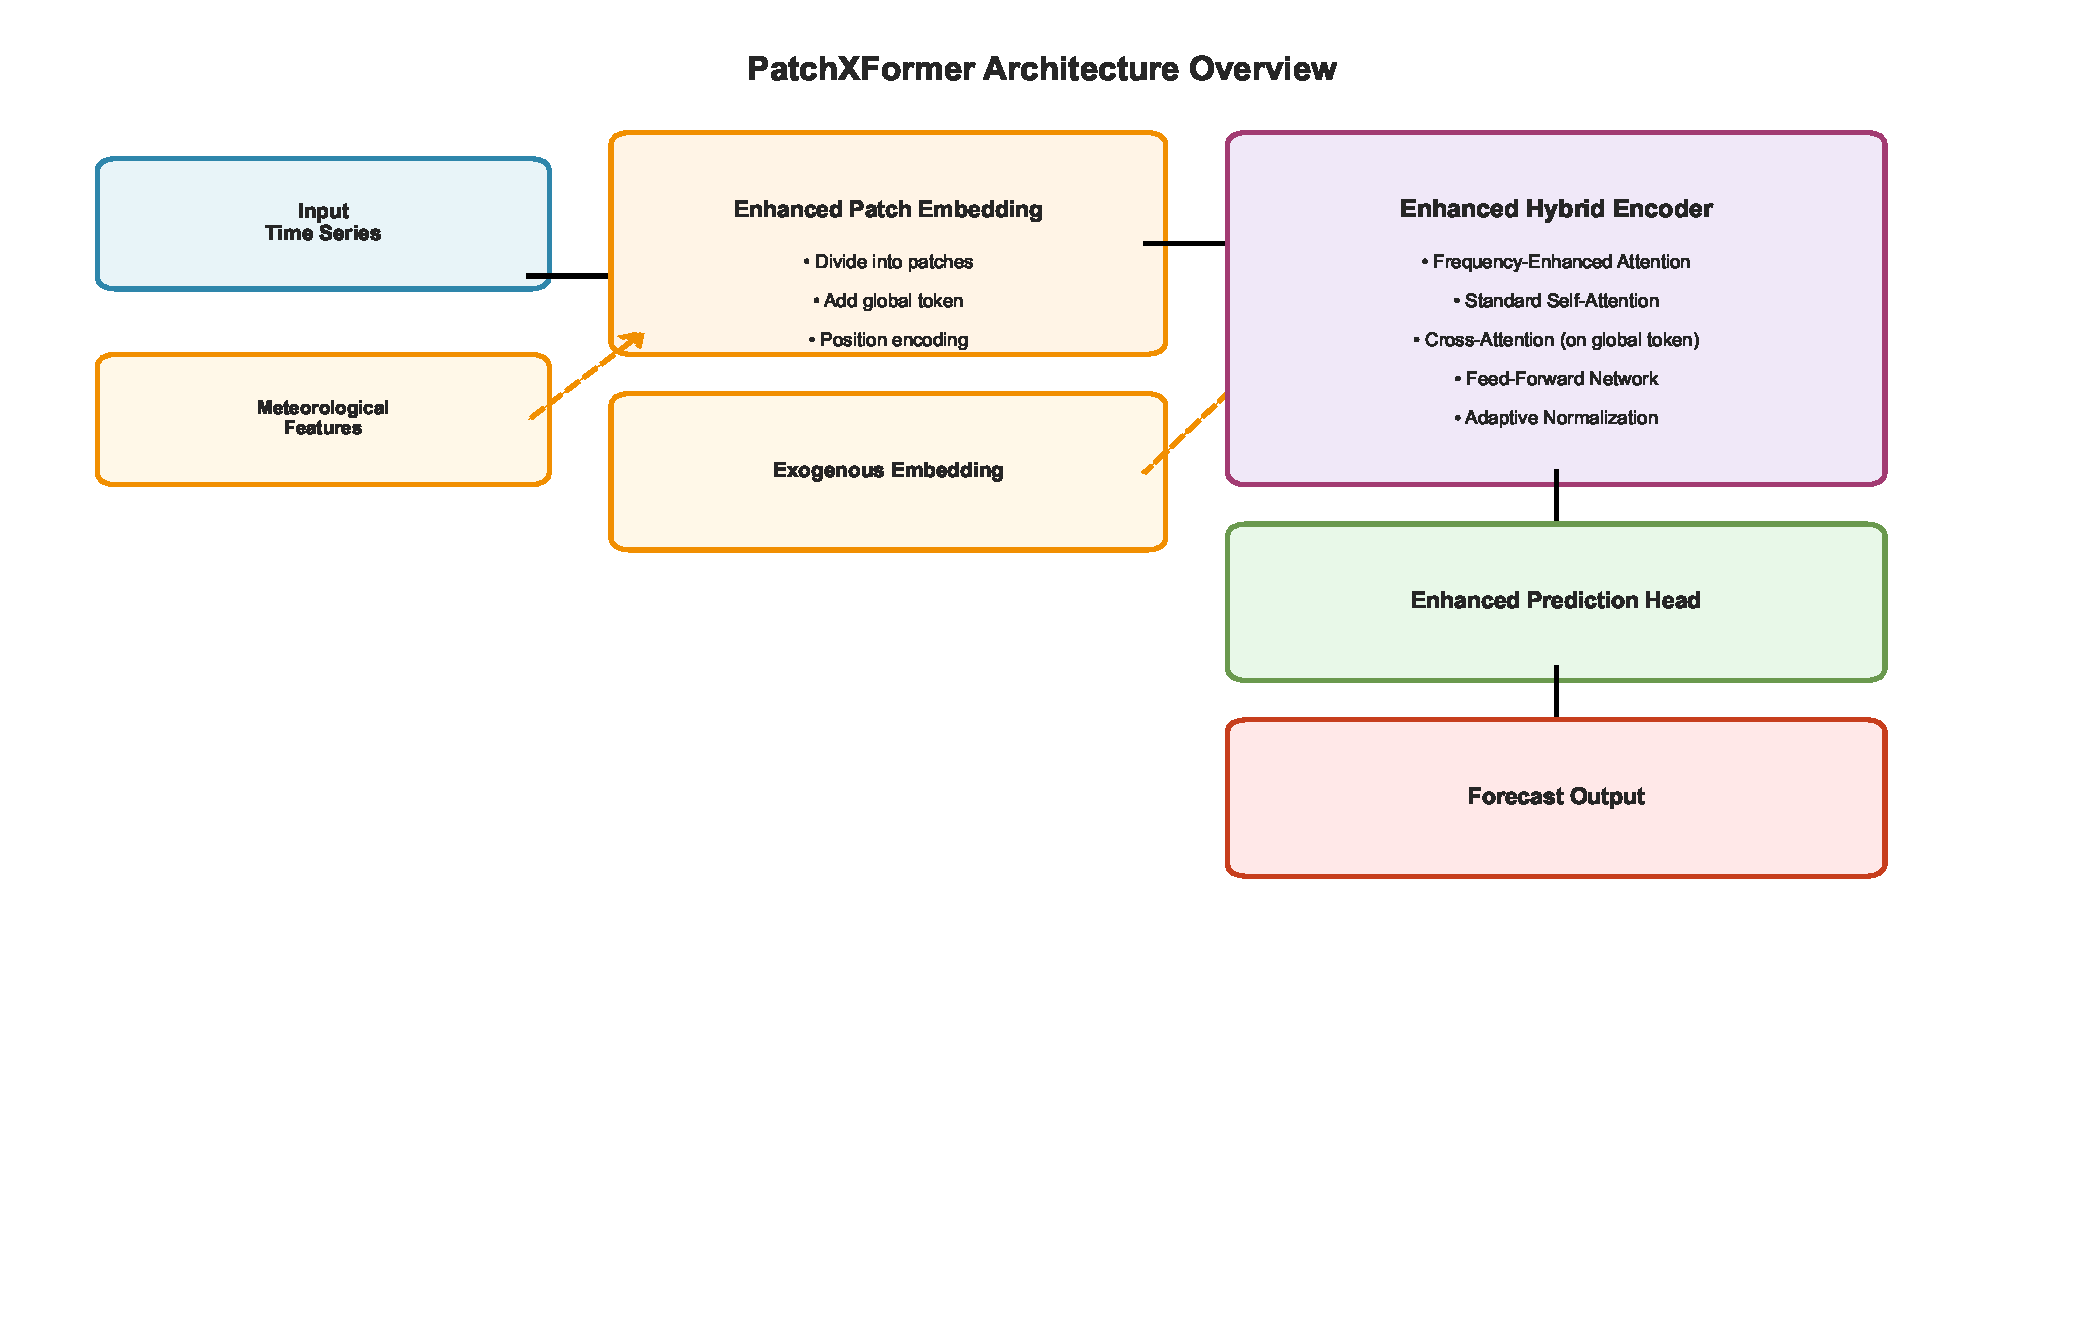
\includegraphics[width=0.85\textwidth]{images/architecture_overview.pdf}
	\caption{Overall architecture of PatchXFormer. The input time series is normalized, divided into patches with global tokens, and processed through encoder layers combining frequency-enhanced attention, standard self-attention, and cross-attention with exogenous features. A linear prediction head generates the final forecast.}
	\label{fig:architecture}
\end{figure*}

\subsection{Enhanced Patch Embedding}

The input time series $X \in \mathbb{R}^{B \times N \times L}$, where $B$ is the batch size, $N$ is the number of variables, and $L$ is the sequence length, is divided into patches of length $P$ with stride $S$:
\begin{equation}
X_{patch} = \text{unfold}(X, \text{size}=P, \text{stride}=S)
\end{equation}
where $X_{patch} \in \mathbb{R}^{B \times N \times P_{num} \times P}$ and $P_{num}$ is the number of patches.

Each patch is embedded into a $d_{model}$-dimensional space using a linear transformation with Xavier uniform initialization:
\begin{equation}
E_{patch} = X_{patch} W_{embed}, \quad W_{embed} \in \mathbb{R}^{P \times d_{model}}
\end{equation}

Sinusoidal positional encoding provides temporal context:
\begin{align}
PE_{(pos, 2i)} &= \sin\left(\frac{pos}{10000^{2i/d_{model}}}\right) \\
PE_{(pos, 2i+1)} &= \cos\left(\frac{pos}{10000^{2i/d_{model}}}\right)
\end{align}

A key innovation is the inclusion of a learnable global token $G \in \mathbb{R}^{1 \times N \times 1 \times d_{model}}$ for each variable, which serves as a summary representation aggregating information across all patches:
\begin{equation}
E_{final} = \text{Dropout}(\text{LayerNorm}([E_{patch}; G]))
\end{equation}

\subsection{Frequency-Enhanced Attention}

Frequency-enhanced attention combines standard self-attention with frequency-domain analysis. For input $X$, queries $Q$, keys $K$, and values $V$ are computed and standard multi-head attention is applied:
\begin{equation}
\text{Attention}(Q, K, V) = \text{softmax}\left(\frac{QK^T}{\sqrt{d_k}}\right)V
\end{equation}

Simultaneously, Fast Fourier Transform (FFT) extracts frequency-domain representations:
\begin{equation}
X_{freq\_time} = \text{IFFT}(\text{FFT}(X))
\end{equation}

The outputs are combined using a learnable weight:
\begin{equation}
\text{Output} = \text{Attention}(Q, K, V) + \alpha \cdot X_{freq\_time}
\end{equation}
where $\alpha$ is a learnable scalar balancing temporal and frequency-domain information. This dual-domain approach captures both temporal dependencies and periodic patterns (daily cycles, seasonal variations) fundamental to solar power data.

\subsection{Adaptive Normalization}

Adaptive normalization improves robustness across different data distributions. For input $X$, the normalized output is:
\begin{equation}
\text{AdaptiveNorm}(X) = \frac{X - \mu}{\sigma} \cdot \alpha_{adapt} + \beta_{adapt}
\end{equation}
where $\alpha_{adapt} = \alpha \cdot (1 + \beta \cdot \tanh(\gamma))$ and $\beta_{adapt} = \beta + \delta \cdot \tanh(\gamma)$. Here $\alpha$, $\beta$, $\gamma$, and $\delta$ are learnable parameters that adapt the normalization to different conditions.

\subsection{Hybrid Encoder Architecture}

Each encoder layer processes input through four stages:

\textbf{(1) Frequency-enhanced self-attention} captures both temporal and frequency-domain patterns:
\begin{equation}
X_1 = \text{AdaptiveNorm}(X + \text{Dropout}(\text{FreqAttention}(X)))
\end{equation}

\textbf{(2) Standard self-attention} models relationships between patches:
\begin{equation}
X_2 = \text{AdaptiveNorm}(X_1 + \text{Dropout}(\text{MultiHead}(X_1, X_1, X_1)))
\end{equation}

\textbf{(3) Cross-attention with exogenous features} integrates meteorological data. Global tokens serve as queries while exogenous features $E_{ex}$ serve as keys and values:
\begin{equation}
G_{updated} = G + \text{Dropout}(\text{CrossAttention}(G, E_{ex}, E_{ex}))
\end{equation}

\textbf{(4) Feed-forward network} applies non-linear transformation with GELU activation:
\begin{equation}
X_{out} = \text{LayerNorm}(X_2 + \text{Dropout}(\text{FFN}(X_2)))
\end{equation}

\subsection{Prediction Head}

A simple linear projection converts encoded representations $H \in \mathbb{R}^{B \times N \times (P_{num}+1) \times d_{model}}$ to forecasts:
\begin{equation}
Y_{pred} = H \cdot W_{out} + b_{out}
\end{equation}
This lightweight design acts as an implicit regularizer, preventing overfitting while preserving accuracy. Our ablation study (Section~\ref{sec:ablation}) demonstrates that this simple head outperforms a more complex residual prediction architecture.

\subsection{Training Procedure}

The model is trained using MSE loss with the Adam optimizer and cosine annealing learning rate schedule. Regularization includes dropout after attention mechanisms, early stopping based on validation loss, and weight decay.

\section{Experimental Study}\label{sec:experiments}

\subsection{Datasets}

Four real-world datasets from different geographic locations are employed. Table~\ref{tab:datasets} summarizes their characteristics. Importantly, all three Sri Lankan datasets were collected specifically for this research, addressing the critical gap of limited tropical region data.

\begin{table*}[width=.9\linewidth,pos=h]
\caption{Summary of datasets used in experimental evaluation. All three Sri Lankan datasets (Piliyandala, Point Pedro, Ja-Ela) were collected specifically for this research.}\label{tab:datasets}
\begin{tabular*}{\tblwidth}{@{} lllllll@{} }
\toprule
\textbf{Dataset} & \textbf{Period} & \textbf{Duration} & \textbf{Interval} & \textbf{Location} & \textbf{Climate} & \textbf{Purpose} \\
\midrule
Piliyandala & Jan 2022--Feb 2024 & $\sim$2 years & 15 min & Sri Lanka & Tropical & Primary \\
Point Pedro & Jun--Nov 2024 & 6 months & 15 min & Sri Lanka & Tropical & Intra-country \\
Ja-Ela & Jun--Nov 2024 & 6 months & 15 min & Sri Lanka & Tropical & Intra-country \\
USA Kansas & 2 years (NSRDB) & 2 years & 15 min & Kansas, USA & Temperate & Cross-region \\
\bottomrule
\end{tabular*}
\end{table*}

\textbf{Piliyandala, Sri Lanka:} The primary dataset was collected from a solar installation near Piliyandala, owned by Eleven Engineering \& Construction (Pvt) Ltd. Meteorological data was sourced from the Department of Meteorology, Sri Lanka. The data spans January 29, 2022 to February 20, 2024, recorded at 15-minute intervals, and includes solar power generation along with temperature, relative humidity, wind speed, wind direction, atmospheric pressure, dew point, and cloud cover.

\textbf{Point Pedro and Ja-Ela, Sri Lanka:} These datasets were collected from sites operated by Solarray Energy (Pvt) Ltd., covering June to November 2024 at 15-minute intervals, and are used to evaluate intra-country generalization.

\textbf{USA Kansas:} Obtained from the National Solar Radiation Database (NSRDB)~\cite{NSRDB} for Kansas, USA, representing a temperate climate region for cross-geographic evaluation.

All datasets underwent consistent preprocessing: missing value handling via linear interpolation, outlier detection using the IQR method, cyclical encoding of temporal features, and instance-level normalization. Data was split chronologically: 70\% training, 10\% validation, 20\% testing.

\subsection{Evaluation Metrics}

Two standard metrics are used:
\begin{equation}
\text{MSE} = \frac{1}{n} \sum_{i=1}^{n} (y_i - \hat{y}_i)^2, \quad
\text{MAE} = \frac{1}{n} \sum_{i=1}^{n} |y_i - \hat{y}_i|
\end{equation}
MSE penalizes larger errors heavily, critical for grid stability. MAE provides robust measures of typical prediction accuracy, less sensitive to outliers.

\subsection{Baseline Models}

PatchXFormer is compared against seven state-of-the-art models: PatchTST~\cite{nie2022patchtst}, ITransformer~\cite{liu2023itransformer}, DLinear~\cite{zeng2023transformers}, TFT~\cite{lim2021temporal}, NLinear~\cite{zeng2023transformers}, Informer~\cite{zhou2021informer}, and Autoformer~\cite{wu2021autoformer}. All baselines use publicly available implementations with hyperparameters tuned on validation data.

\subsection{Experimental Setup}

PatchXFormer is configured with: patch length 16, stride 8 (50\% overlap), $d_{model}=128$, 8 attention heads, 3 encoder layers, feed-forward dimension 512, dropout 0.1, learning rate $10^{-4}$ with cosine annealing, batch size 64, and 100 training epochs with early stopping (patience 5). Experiments evaluate four forecasting horizons: 96 (24h), 192 (48h), 336 (3.5 days), and 720 (7.5 days) time steps, with input sequence length fixed at 96 steps.

\subsection{Results on Piliyandala Dataset}

Table~\ref{tab:main_results} presents the primary comparison of PatchXFormer with baselines across all forecasting horizons on the Piliyandala dataset.

\begin{table*}[width=.9\linewidth,pos=h]
\caption{Evaluation on the Piliyandala dataset. Input sequence length is 96. Best results in bold.}\label{tab:main_results}
\begin{tabular*}{\tblwidth}{@{} lcccccccccccccc@{} }
\toprule
\textbf{Models} & \multicolumn{2}{c}{\textbf{PatchXFormer}} & \multicolumn{2}{c}{\textbf{PatchTST}} & \multicolumn{2}{c}{\textbf{ITransformer}} & \multicolumn{2}{c}{\textbf{DLinear}} & \multicolumn{2}{c}{\textbf{TFT}} & \multicolumn{2}{c}{\textbf{NLinear}} & \multicolumn{2}{c}{\textbf{Informer}} \\
\textbf{Metric} & \textbf{MSE} & \textbf{MAE} & \textbf{MSE} & \textbf{MAE} & \textbf{MSE} & \textbf{MAE} & \textbf{MSE} & \textbf{MAE} & \textbf{MSE} & \textbf{MAE} & \textbf{MSE} & \textbf{MAE} & \textbf{MSE} & \textbf{MAE} \\
\midrule
\textbf{96}  & \textbf{0.201} & \textbf{0.253} & 0.216 & 0.265 & 0.214 & 0.267 & 0.250 & 0.312 & 0.253 & 0.292 & 0.251 & 0.295 & 0.253 & 0.312\\
\textbf{192} & \textbf{0.233} & \textbf{0.279} & 0.247 & 0.288 & 0.244 & 0.288 & 0.332 & 0.390 & 0.303 & 0.322 & 0.283 & 0.318 & 0.346 & 0.391\\
\textbf{336} & \textbf{0.257} & \textbf{0.297} & 0.272 & 0.306 & 0.272 & 0.306 & 0.367 & 0.420 & 0.351 & 0.350 & 0.309 & 0.335 & 0.433 & 0.466\\
\textbf{720} & \textbf{0.295} & \textbf{0.320} & 0.315 & 0.332 & 0.312 & 0.331 & 0.425 & 0.462 & 0.437 & 0.394 & 0.349 & 0.359 & 0.697 & 0.591\\
\bottomrule
\end{tabular*}
\end{table*}

PatchXFormer achieves the best performance across all forecasting horizons. For the 96-step horizon, PatchXFormer achieves MSE of 0.201 and MAE of 0.253, representing improvements of 6.1\% and 5.2\% over ITransformer (the second-best model). At the 720-step horizon, PatchXFormer maintains its advantage with MSE of 0.295 and MAE of 0.320, achieving improvements of 5.4\% and 3.3\% over ITransformer. The consistent advantage across all horizons demonstrates PatchXFormer's robustness for both short-term and long-term forecasting.

As expected, forecasting accuracy decreases with longer horizons. PatchXFormer experiences an absolute MSE increase of 0.094 from 96-step to 720-step, while maintaining a 5.4\% improvement over the best baseline at the longest horizon.

\subsection{Cross-Geographic Evaluation}

\subsubsection{USA Kansas Dataset Results}

Table~\ref{tab:us_results} compares PatchXFormer performance on the USA Kansas dataset against the Piliyandala dataset.

\begin{table}[width=.9\linewidth,pos=h]
\caption{PatchXFormer performance comparison: USA Kansas vs.\ SL Piliyandala (within-region evaluation).}\label{tab:us_results}
\begin{tabular*}{\tblwidth}{@{} lcccc@{} }
\toprule
\textbf{Horizon} & \multicolumn{2}{c}{\textbf{USA Kansas}} & \multicolumn{2}{c}{\textbf{SL Piliyandala}} \\
 & \textbf{MSE} & \textbf{MAE} & \textbf{MSE} & \textbf{MAE} \\
\midrule
\textbf{96}  & 0.157 & 0.217 & 0.201 & 0.253\\
\textbf{192} & 0.214 & 0.275 & 0.233 & 0.279\\
\textbf{336} & 0.251 & 0.309 & 0.257 & 0.297\\
\textbf{720} & 0.294 & 0.340 & 0.295 & 0.320\\
\bottomrule
\end{tabular*}
\end{table}

PatchXFormer achieves generally better performance on the USA Kansas dataset, attributable to the more predictable weather patterns in temperate climates compared to the high humidity, significant cloud cover variability, and distinct wet/dry seasons of tropical Sri Lanka.

\subsubsection{Cross-Region Evaluation}

Table~\ref{tab:cross_region} presents cross-region evaluation results where models trained on one region are tested on another.

\begin{table*}[width=.9\linewidth,pos=h]
\caption{Cross-region evaluation results showing performance degradation across geographic regions.}\label{tab:cross_region}
\begin{tabular*}{\tblwidth}{@{} llcccc@{} }
\toprule
\textbf{Training} & \textbf{Testing} & \textbf{96-step} & \textbf{192-step} & \textbf{336-step} & \textbf{720-step} \\
 &  & \textbf{MSE/MAE} & \textbf{MSE/MAE} & \textbf{MSE/MAE} & \textbf{MSE/MAE} \\
\midrule
USA Kansas & USA Kansas & 0.157/0.217 & 0.214/0.275 & 0.251/0.309 & 0.294/0.340\\
SL Piliyandala & SL Piliyandala & 0.201/0.253 & 0.233/0.279 & 0.257/0.297 & 0.295/0.320\\
USA Kansas & SL Piliyandala & 4.043/0.771 & 4.938/0.865 & 6.125/0.953 & 7.332/1.045\\
SL Piliyandala & USA Kansas & 0.275/0.267 & 0.381/0.316 & 0.439/0.343 & 0.496/0.375\\
\bottomrule
\end{tabular*}
\end{table*}

The cross-region evaluation reveals a striking asymmetry in geographic generalization. When PatchXFormer trained on USA Kansas data is tested on SL Piliyandala data, MSE increases dramatically to 4.043 (96-step), a 25.8-fold increase. Conversely, when trained on SL Piliyandala and tested on USA Kansas, MSE increases to 0.275, only a 36.8\% increase. This asymmetric pattern suggests that training on the more variable tropical conditions forces the model to learn more robust and adaptable patterns that transfer better to the relatively more stable temperate conditions.

\subsubsection{Intra-Country Evaluation}

Table~\ref{tab:intra_country} presents results when models trained on Piliyandala data are tested on other Sri Lankan locations.

\begin{table}[width=.9\linewidth,pos=h]
\caption{Intra-country evaluation: models trained on Piliyandala, tested on other Sri Lankan locations.}\label{tab:intra_country}
\begin{tabular*}{\tblwidth}{@{} lcccc@{} }
\toprule
\textbf{Testing} & \textbf{96-step} & \textbf{192-step} & \textbf{336-step} & \textbf{720-step} \\
\textbf{Location} & \textbf{MSE/MAE} & \textbf{MSE/MAE} & \textbf{MSE/MAE} & \textbf{MSE/MAE} \\
\midrule
Point Pedro & 0.319/0.289 & 0.398/0.331 & 0.466/0.362 & 0.546/0.403\\
Ja-Ela & 0.225/0.267 & 0.267/0.299 & 0.297/0.322 & 0.329/0.345\\
\bottomrule
\end{tabular*}
\end{table}

Performance on Ja-Ela (MSE: 0.225 for 96-step) is better than on Point Pedro (MSE: 0.319), explained by geographic proximity and climatic similarity. Ja-Ela is in the same Western Province as Piliyandala, sharing similar rainfall and cloud cover patterns. Point Pedro, in the Northern Province, experiences a drier climate, creating a more challenging distribution shift. The degradation is much smaller than cross-country degradation, indicating models generalize reasonably within similar climatic regions.

\subsection{Feature Importance Analysis}

Table~\ref{tab:feature_importance} compares PatchXFormer performance with and without meteorological features.

\begin{table}[width=.9\linewidth,pos=h]
\caption{Feature importance analysis: performance with and without meteorological features on Piliyandala dataset.}\label{tab:feature_importance}
\begin{tabular*}{\tblwidth}{@{} lcccc@{} }
\toprule
\textbf{Configuration} & \textbf{96-step} & \textbf{192-step} & \textbf{336-step} & \textbf{720-step} \\
 & \textbf{MSE/MAE} & \textbf{MSE/MAE} & \textbf{MSE/MAE} & \textbf{MSE/MAE} \\
\midrule
With Weather & 0.201/0.253 & 0.233/0.279 & 0.257/0.297 & 0.295/0.320\\
Without Weather & 0.242/0.264 & 0.257/0.276 & 0.268/0.285 & 0.307/0.296\\
\bottomrule
\end{tabular*}
\end{table}

Including meteorological features improves accuracy, particularly for shorter horizons: 16.9\% MSE reduction for 96-step but only 4.1\% for 720-step. This suggests weather features are more valuable for short-term forecasting where current conditions have direct impact, while longer-term forecasts rely more on learned temporal patterns. Interestingly, the model without weather data shows more stable performance across horizons (26.8\% MSE increase from 96 to 720-step vs.\ 46.8\% with weather data), suggesting that weather features introduce variability that becomes harder to predict over longer horizons.

\subsection{Ablation Study}\label{sec:ablation}

A comprehensive ablation study evaluates the contribution of each architectural component through progressive enhancement from a baseline.

\begin{table*}[width=.9\linewidth,pos=h]
\caption{Ablation study results on Piliyandala dataset. Variant 4 achieves the best overall performance and is selected as the final architecture.}\label{tab:ablation}
\begin{tabular*}{\tblwidth}{@{} lcccc@{} }
\toprule
\textbf{Variant} & \textbf{96-step} & \textbf{192-step} & \textbf{336-step} & \textbf{720-step} \\
 & \textbf{MSE/MAE} & \textbf{MSE/MAE} & \textbf{MSE/MAE} & \textbf{MSE/MAE} \\
\midrule
Variant 0 (Baseline) & 0.217/0.266 & 0.246/0.288 & 0.272/0.309 & 0.314/0.331\\
Variant 1 (+Enhanced Patch) & 0.207/0.256 & 0.240/0.284 & 0.269/0.302 & 0.307/0.326\\
Variant 2 (+Frequency Attn.) & 0.210/0.260 & 0.244/0.288 & 0.265/0.300 & 0.306/0.330\\
Variant 3 (+Adaptive Norm.) & 0.209/0.258 & 0.243/0.286 & 0.264/0.298 & 0.304/0.329\\
\textbf{Variant 4 (+Cross-Attn.)} & \textbf{0.201/0.253} & \textbf{0.233/0.279} & \textbf{0.257/0.297} & \textbf{0.295/0.320}\\
Variant 5 (+Residual Head) & 0.205/0.256 & 0.232/0.278 & 0.259/0.298 & 0.307/0.327\\
\bottomrule
\end{tabular*}
\end{table*}

The ablation study (Table~\ref{tab:ablation}) reveals several key findings:

\begin{enumerate}
\item \textbf{Cross-attention is critical:} Adding cross-attention for exogenous feature integration (Variant 4) provides the largest single improvement---an additional 4\% MSE reduction for 96-step compared to Variant 3. This demonstrates the importance of effectively leveraging meteorological data through specialized attention mechanisms.

\item \textbf{Enhanced patch embedding provides foundation:} Global tokens and improved initialization achieve 4.6\% MSE reduction for 96-step over the baseline, providing consistent improvements across all horizons.

\item \textbf{Frequency enhancement aids long-term prediction:} While frequency-enhanced attention shows marginal improvement on shorter horizons, it provides more benefit for longer horizons (336 and 720 steps), suggesting frequency-domain analysis is particularly valuable for capturing long-term periodic patterns.

\item \textbf{Adaptive normalization provides modest gains:} The contribution is relatively modest compared to cross-attention, though it helps maintain robustness across different conditions.

\item \textbf{Residual prediction head degrades performance:} Surprisingly, adding residual connections to the prediction head (Variant 5) degrades performance, particularly on longer horizons (MSE increases from 0.295 to 0.307 for 720-step). The simpler linear head provides better generalization.
\end{enumerate}

Based on these results, Variant 4 is selected as the final PatchXFormer architecture, achieving the optimal balance between performance and complexity.

\section{Discussion}\label{sec:discussion}

\subsection{Architectural Effectiveness}

The experimental results demonstrate that PatchXFormer's architectural innovations---enhanced patch embedding, frequency-enhanced attention, adaptive normalization, and cross-attention---effectively improve SPG forecasting accuracy. The consistent improvements across all horizons, particularly the 5.4\% MSE improvement at the 720-step horizon over the best baseline, validate the design choices for long-term forecasting.

The ablation study reveals that cross-attention for meteorological feature integration provides the largest performance gain. This finding is significant: while most existing Transformer variants treat all inputs uniformly, PatchXFormer's specialized cross-attention mechanism enables more effective leveraging of weather data, which is the dominant factor influencing solar power generation.

\subsection{Geographic Generalization}

The cross-geographic evaluation reveals two important patterns. First, geographic generalization across different climatic zones remains a significant challenge, with models showing substantial performance degradation when applied across regions. Second, the asymmetric generalization---models trained on tropical data generalize better to temperate regions than vice versa---provides a novel finding. The more variable tropical conditions (high humidity, significant cloud cover variability, distinct wet/dry seasons) appear to force models to learn more robust representations that transfer better to more predictable temperate environments.

The intra-country results demonstrate that geographic proximity and climatic similarity significantly influence generalization quality. Models maintain reasonable performance within similar climatic regions, supporting regional deployment strategies where data from nearby locations can supplement limited local data.

\subsection{Feature Importance}

The finding that meteorological features provide decreasing benefit for longer horizons reveals a fundamental characteristic of SPG forecasting: current weather conditions have direct, predictable impact on short-term generation, while longer-term predictions depend more on learned temporal patterns (diurnal and seasonal cycles) that the model captures through its frequency-enhanced attention mechanism. This insight provides practical guidance: for short-term applications, investing in high-quality weather data is valuable; for long-term planning, temporal pattern modeling may be more important.

\subsection{Comparison with Existing Work}

PatchXFormer advances beyond prior work in several ways. Compared to PatchTST, it adds frequency-domain analysis and specialized meteorological feature integration. Unlike Informer's sparse attention, PatchXFormer maintains full attention with frequency enhancement, better capturing structured periodic patterns. While Autoformer assumes clean decomposition, PatchXFormer flexibly learns patterns through combined temporal-frequency attention. Against TFT, PatchXFormer achieves 32.5\% lower MSE for the 720-step horizon with a simpler architecture.

\subsection{Limitations}

Several limitations should be acknowledged: (1) geographic coverage is limited to tropical (Sri Lanka) and temperate (USA) climates; (2) some datasets have limited temporal coverage (6 months); (3) PatchXFormer's enhanced architecture increases computational requirements; (4) the evaluation uses MSE and MAE only; and (5) real-world deployment challenges such as data latency and model drift are not addressed. Future work should expand geographic diversity, investigate transfer learning for cross-region deployment, and explore probabilistic forecasting extensions.

\section{Conclusion}\label{sec:conclusion}

This paper proposed PatchXFormer, a novel Transformer-based architecture for long-term solar power generation forecasting. PatchXFormer incorporates enhanced patch embedding with global tokens, frequency-enhanced attention mechanisms, adaptive normalization, and cross-attention for exogenous feature integration. Comprehensive experiments across four real-world datasets from two climatic regions demonstrate consistent improvements over seven state-of-the-art baselines, with MSE improvements of 6.1\% (24h horizon) to 5.4\% (7.5-day horizon) on the primary dataset.

The research contributes three new real-world datasets from tropical Sri Lanka, addressing a critical data gap. The ablation study validates that cross-attention for meteorological feature integration provides the largest performance gain, while a simpler linear prediction head outperforms a more complex residual architecture. Cross-geographic evaluation reveals significant generalization challenges across climatic zones, with an interesting asymmetric pattern where tropical-trained models generalize better to temperate regions than vice versa. Intra-country evaluation demonstrates more robust generalization within similar climatic conditions.

Future research directions include transfer learning for cross-geographic deployment, probabilistic forecasting extensions, integration with energy management systems, and extended evaluation across diverse climatic regions.

\section*{Declaration of competing interest}

The authors declare that they have no known competing financial interests or personal relationships that could have appeared to influence the work reported in this paper.

\section*{Data availability}

The datasets used in this study are publicly available at the following GitHub repository: \url{https://github.com/chathushka1996/Solar-Power-Generation-Forecasting}.

\section*{Acknowledgements}

The authors would like to thank Eleven Engineering \& Construction (Pvt) Ltd.\ and Solarray Energy (Pvt) Ltd.\ for providing access to solar power generation data, and the Department of Meteorology, Sri Lanka for meteorological data.

\section*{CRediT authorship contribution statement}

\printcredits

\bibliographystyle{cas-model2-names}
\bibliography{references}

\end{document}
